\documentclass[11pt]{article}
% default ORG mode 
\usepackage[utf8]{inputenc}  \usepackage[T1]{fontenc} \usepackage{fixltx2e}
\usepackage{graphicx}        \usepackage{longtable}   \usepackage{float}
\usepackage{wrapfig}         \usepackage{soul}        \usepackage{textcomp}
\usepackage{marvosym}        \usepackage{wasysym}     \usepackage{latexsym}
\usepackage{amsmath}         \usepackage{amssymb}     \usepackage{color}
\usepackage{rotating}        \usepackage{hyperref}    \usepackage{xcolor} 
\usepackage{palatino}
% my customizations
\usepackage{enumitem}
\usepackage{amsthm}
\tolerance=1000
%\providecommand{\alert}[1]{\textbf{#1}}
\usepackage[top=1in, bottom=1in, left=1in, right=1in]{geometry}

\title{Dodson \& Poston Exercise VII.2.3: concrete example}
\author{Peter Mao, $\ldots$}
\date{\today}

\begin{document}

\maketitle
\pagestyle{empty}

\begin{abstract}
  It may be helpful to have a concrete example to understand the equivalence
  relation in Exercise VII.2.3a.
\end{abstract}

\section{Introduction}

This excercise establishes an equivalence relation between tangent vectors of
overlapping charts:

\begin{quote}
  Let $(U,\phi)$, $(U',\phi')$ be charts on a smooth manifold $M$, modelled on
  an affine space $X$ with vector space $T$, $u \in U \cap U'$, and $\vec{t},
  \vec{t'} \in T$. Define the relation $\sim$ by

  \[
  (U, \phi, \vec{t}) \sim (U', \phi', \vec{t'}) \iff D_{\phi(u)}(\phi' \circ
  \phi^{\leftarrow}\vec{t}) = \vec{t'}
  \]
\end{quote}

In the following section, I concretely demonstrate symmetry of this equivalence
relation using two charts on the unit circle ($S^1$).

\section{Example with $S^1$}

Table~\ref{Tbl:defns} summarizes the concrete elements and
Figure~\ref{Fig:defns} gives a visual representation of this example.


\begin{table}[h]
\begin{center}
\caption{Elements of this example in relation to the symbols of Exercise VII.2.3.}
\label{Tbl:defns}
\begin{tabular}{|l|l|l|} \hline
  D\&P & here & comments \\ \hline
  $M$ & $S^1$    & the unit circle in $\mathbb{C}$ or $\mathbb{R}$, parameterized by $\theta$ \\
  $X$ & $(X, Y)$ & $\mathbb{R^2}$, the affine space on which $M$ is modelled \\
  $U$ & $U_{Y+}$ & the open semicircle in $Y > 0$ \\
  $\phi$ & $\cos\theta = x$ & projection onto $X$\\
  $U'$ & $U_{X+}$ & the open semicircle in $X > 0$ \\
  $\phi'$ & $\sin\theta = y$ & projection onto $Y$\\ \hline
\end{tabular}
\end{center}
\end{table}

\begin{figure}[h]
\centerline{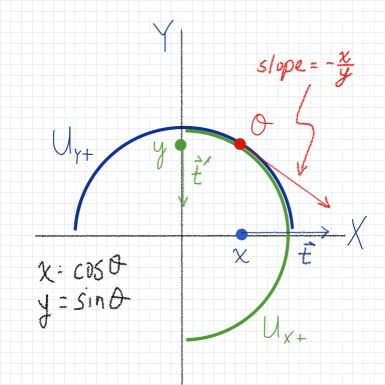
\includegraphics[height=3.25in,angle=0]{figs/Ex.VII.2.3_1_PHM.png}}
\caption{\small{Charts on $\protect S^1$ used in this example.}}
\label{Fig:defns}
\end{figure}


For reference, here are some relevant  not-so-often used derivatives:
\begin{align}
  \frac{d}{dx}\arccos x &= -\frac{1}{\sqrt{1 - x^2}} \\
  \frac{d}{dx}\arcsin x &= \frac{1}{\sqrt{1 - x^2}}.
\end{align}
For the triplet $(U_{Y+}, \cos\theta, \vec{t}=1)$, we can solve for $\vec{t'}$ by
the definition given:
\begin{align}
  \vec{t'} &= D_x(\sin \circ \arccos) \\
  &= D_{\arccos x}\sin \circ D_x \arccos              \label{Eqn:chain} \\
  &= \cos(\arccos x) \cdot -\frac{1}{\sqrt{1 - x^2}} \label{Eqn:prod} \\
  &= -\frac{x}{\sqrt{1 - x^2}} \\
  &= -\frac{x}{y}.
\end{align}
In going from Equation~\ref{Eqn:chain} to Equation~\ref{Eqn:prod}, recall that
the composition in Equation~\ref{Eqn:chain} is a composition of linear maps (ie,
matrices), and that in one dimension, the composition of linear maps reduces to
standard mulitiplication of real numbers.  For $(U_{X+}, \sin\theta,
\vec{t'}=1)$ we can solve for $\vec{t}$ in the same way:
\begin{align}
  \vec{t} &= D_y(\cos \circ \arcsin) \\
  &= D_{\arcsin y}\cos \circ D_y \arcsin \\
  &= -\sin(\arcsin y) \cdot \frac{1}{\sqrt{1 - y^2}} \\
  &= -\frac{y}{\sqrt{1 - y^2}} \\
  &= -\frac{y}{x}.
\end{align}
So, in this concrete example, we have the equivalence relations
\begin{align}
  (U_{Y+}, \cos\theta, 1) &\sim \bigg(U_{X+}, \sin\theta, -\frac{x}{y}\bigg) \\
  (U_{X+}, \sin\theta, 1) &\sim \bigg(U_{Y+}, \cos\theta, -\frac{y}{x}\bigg)
\end{align}
from which we can check symmetry:
\begin{align}
    \bigg(U_{X+}, \sin\theta, -\frac{x}{y}\bigg) &\sim \bigg(U_{Y+}, \cos\theta, \bigg(-\frac{y}{x}\bigg)\bigg(-\frac{x}{y}\bigg)\bigg) \\
&\sim (U_{Y+}, \cos\theta, 1).
\end{align}

Transitivity cannot be checked with this example because we don't have three
easily overlapping charts.  Using $S^2$, the unit sphere, we could follow the
same procedures to establish transitivity in a concrete example.

\end{document}



%% commonly used blocks
\begin{quote}
\end{quote}

\begin{proof}
\end{proof}

\begin{align}
\end{align}

\begin{equation}
\end{equation}

\begin{remark}
\end{remark}

